% !TEX root = ../main_hessenberg.tex
\section{Case study: Digraphs of real-orthogonal upper Hessenberg matrices}\label{sec:example}
We work with $n \times n$ real matrices ($n \ge 2$), indexed by
$[n] = \{1, 2, \dots, n\}$.

\begin{definition}[Orthogonal upper Hessenberg matrix]\label{def:OH}
\leanmargin{OrthogonalHessenberg}{Matrix/OrthogonalHessenberg.lean\#L67}
A matrix $Q \in \R^{n \times n}$ is \emph{upper Hessenberg} if $Q_{ij} = 0$
whenever $j + 1 < i$, and \emph{orthogonal} if $Q^\top Q = \Id$. We write
$\mathcal{H}_n$ for the set of orthogonal upper Hessenberg matrices in
$\R^{n \times n}$.
\end{definition}

\begin{definition}[Support digraph]\label{def:support}
\leanmargin{supportDigraph}{Matrix/SupportDigraph.lean\#L37}
The \emph{support digraph} of an $n \times n$ real matrix $Q$, denoted $D(Q)$,
is the directed graph on $[n]$ with an arc $i \to j$ whenever $Q_{ij} \ne 0$.
Figure~\ref{fig:intro-example} illustrates a small instance.
\end{definition}

\begin{figure}[htbp]
\centering
\begin{tikzpicture}[
  v/.style={circle, draw=black, line width=0.6pt, inner sep=1.2pt,
            minimum size=18pt, font=\small},
  arr/.style={-{Stealth[length=5pt]}, line width=0.8pt, draw=black},
]
% Matrix on the left
\node (mat) at (-2.5, 0) {$Q = \begin{pmatrix}
\bullet & \bullet & 0 & \bullet \\
\bullet & \bullet & 0 & \bullet \\
0 & \bullet & 0 & 0 \\
0 & 0 & \bullet & 0
\end{pmatrix}$};

% Arrow from matrix to digraph
\draw[-{Stealth[length=5pt]}, thick] (0.6, 0) -- (1.8, 0)
  node[midway, above, font=\footnotesize] {$D(Q)$};

% Digraph on the right (square layout, centered)
\node[v] (1) at (3.0, 1.0)  {1};
\node[v] (2) at (5.0, 1.0)  {2};
\node[v] (3) at (5.0, -1.0) {3};
\node[v] (4) at (3.0, -1.0) {4};

\draw[arr, loop above, looseness=8, min distance=8mm] (1) to (1);
\draw[arr, loop above, looseness=8, min distance=8mm] (2) to (2);
\draw[arr, bend left=12] (1) to (2);
\draw[arr, bend left=12] (2) to (1);
\draw[arr] (1) to (4);
\draw[arr] (2) to (4);
\draw[arr] (3) to (2);
\draw[arr] (4) to (3);
\end{tikzpicture}
\caption{A $4 \times 4$ upper Hessenberg matrix ($\bullet$ = nonzero) and its
support digraph $D(Q)$. Each nonzero entry $Q_{ij}$ becomes a directed arc
$i \to j$.}
\label{fig:intro-example}
\end{figure}
\FloatBarrier

\begin{definition}[Sign-equivalence]\label{def:sign}
\leanmargin{SignEquiv}{Matrix/SignEquivalence.lean\#L71}
Two matrices $Q, Q' \in \R^{n \times n}$ are \emph{sign-equivalent},
written $Q \simeq_{\mathrm{sign}} Q'$, if $Q' = D_L\, Q\, D_R$ for some
\emph{signature matrices} $D_L, D_R$ --- diagonal matrices whose diagonal
entries are all $\pm 1$.
\end{definition}

\begin{corollary}[Sign-invariance of the support digraph]\label{cor:sign-support}
\leanmargin{supportDigraph\_eq\_of\_signEquiv}{Matrix/SignEquivalence.lean\#L184}
Sign-equivalent matrices have identical zero / non-zero patterns; hence
$D(Q) = D(Q')$ whenever $Q \simeq_{\mathrm{sign}} Q'$.
\end{corollary}

\begin{definition}[Givens rotation, ordered Givens product]\label{def:givens}
\leanmargintwo{givensRotation}{Matrix/Givens/Rotation.lean\#L67}{givensProduct}{Matrix/Givens/Product.lean\#L69}
For $k \in \{0, \dots, n-2\}$ and $\theta \in \R$, the \emph{Givens rotation}
$G_k(\theta) \in \R^{n \times n}$ is the identity with the $2 \times 2$
block at rows / columns $(k, k{+}1)$ replaced by
$\bigl[\begin{smallmatrix}\cos\theta & -\sin\theta\\ \sin\theta & \cos\theta\end{smallmatrix}\bigr]$.
The \emph{ordered Givens product} of an angle vector $\theta = (\theta_0,
\dots, \theta_{n-2})$ is
\[
  Q_n(\theta) \;\defeq\; G_0(\theta_0)\, G_1(\theta_1)\,\cdots\,G_{n-2}(\theta_{n-2}).
\]
The product $Q_n(\theta)$ is always orthogonal upper Hessenberg, and its
$(k{+}1, k)$ subdiagonal entry equals $\sin\theta_k$.
\end{definition}

The angle vector is called \emph{unreduced} if every $\sin\theta_k$ is
non-zero; equivalently, every subdiagonal entry of $Q_n(\theta)$ is
non-zero. We write $\Theta_n$ for the set of such unreduced angle vectors.

\begin{definition}[Active set, combinatorial digraph]\label{def:active-set}
\leanmargintwo{ActiveSet}{ActiveSet.lean\#L70}{digraph}{ActiveSet.lean\#L281}
An \emph{active set} is any subset $S \subseteq [n-1]$. From $S$ we derive
\[
  R(S) \;\defeq\; \{1\} \cup \{k+1 : k \in S\}, \qquad
  C(S) \;\defeq\; S \cup \{n\}
\]
(\emph{active rows} / \emph{active columns}), and the \emph{combinatorial
digraph} $D_n(S)$ on $[n]$, whose arcs are of two kinds: \emph{spine} arcs
$j+1 \to j$ for $1 \le j \le n-1$, and \emph{overlay} arcs $i \to j$ whenever
$i \in R(S)$, $j \in C(S)$, and $i \le j$. This construction uses the set $S$
alone; no matrix or angle vector enters.

The \emph{active set of an angle vector} $\theta \in \Theta_n$ is
\[
  S(\theta) \;\defeq\; \bigl\{\, k+1 \,:\, k \in \{0, \dots, n-2\},\ \cos\theta_k \ne 0\,\bigr\} \;\subseteq\; [n-1],
\]
the subset to which $D_n$ is applied on the matrix side.
\end{definition}

\begin{example}[$n = 6$, $S = \{2, 4\}$ — anatomy of $D_6(\{2,4\})$]\label{ex:D6S24}
\leanmargin{example\_D6\_S24}{PaperExamples.lean\#L67}
The angle vector $\theta = (\pi/2, \pi/4, \pi/2, \pi/4, \pi/2)$ produces
$\cos\theta_k \ne 0$ exactly for $k \in \{1, 3\}$, hence
$S = \{2, 4\}$. The active rows and columns are
\[
  R = \{1, 3, 5\}, \qquad C = \{2, 4, 6\},
\]
and the resulting digraph $D_6(\{2, 4\})$ is depicted in
Figure~\ref{fig:digraph-anatomy}: the spine cycle in solid black and the
overlay arcs as dashed blue edges from $R$ to $C$. Here $R \cap C =
\emptyset$, so $D_6(\{2, 4\})$ has no self-loops.
\end{example}

\begin{figure}[htbp]
\centering
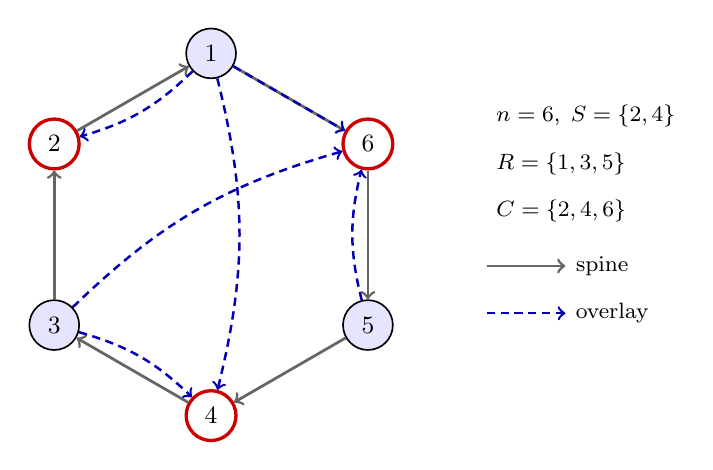
\begin{tikzpicture}[
  v/.style={circle, draw=black, line width=0.6pt, inner sep=1.2pt,
            minimum size=18pt, font=\small},
  spine/.style={->, line width=1.0pt, draw=black!60},
  over/.style={->, line width=0.9pt, draw=blue!70!black, densely dashed},
  Rnode/.style={fill=blue!10},
  Cnode/.style={draw=red!80!black, line width=1.2pt},
  RCnode/.style={fill=blue!10, draw=red!80!black, line width=1.2pt}
]
% n=6, S={2,4}
\def\radius{2.3}
\node[v,Rnode]  (1) at (90:\radius)  {1};
\node[v,Cnode]  (6) at (30:\radius)  {6};
\node[v,Rnode]  (5) at (-30:\radius) {5};
\node[v,Cnode]  (4) at (-90:\radius) {4};
\node[v,Rnode]  (3) at (-150:\radius){3};
\node[v,Cnode]  (2) at (150:\radius) {2};

% Spine (Hamilton cycle)
\draw[spine] (1) -- (6) node[midway, above right, font=\scriptsize, black!60] {};
\draw[spine] (6) -- (5);
\draw[spine] (5) -- (4);
\draw[spine] (4) -- (3);
\draw[spine] (3) -- (2);
\draw[spine] (2) -- (1);

% Overlay arcs: i in R={1,3,5}, j in C={2,4,6}, i <= j
\draw[over, bend left=14] (1) to (2);
\draw[over, bend left=14] (1) to (4);
\draw[over] (1) to (6);
\draw[over, bend left=14] (3) to (4);
\draw[over, bend left=14] (3) to (6);
\draw[over, bend left=14] (5) to (6);

% Legend
\node[anchor=west, font=\footnotesize] at (3.5, 1.5) {$n = 6,\; S = \{2, 4\}$};
\node[anchor=west, font=\footnotesize] at (3.5, 0.9) {$R = \{1, 3, 5\}$};
\node[anchor=west, font=\footnotesize] at (3.5, 0.3) {$C = \{2, 4, 6\}$};
\draw[spine] (3.5, -0.4) -- (4.5, -0.4)
  node[right, font=\footnotesize] {spine};
\draw[over] (3.5, -1.0) -- (4.5, -1.0)
  node[right, font=\footnotesize] {overlay};
\end{tikzpicture}
\caption{Anatomy of $D_6(\{2,4\})$. Solid arrows form the directed Hamilton
cycle (spine). Dashed blue arrows are the overlay arcs from active rows
$R = \{1,3,5\}$ (blue fill) to active columns $C = \{2,4,6\}$ (red outline).
Self-loops occur exactly at vertices in $R \cap C$; here $R \cap C =
\emptyset$, so $D_6(\{2,4\})$ is loopless.}
\label{fig:digraph-anatomy}
\end{figure}
\FloatBarrier

\begin{theorem}[Universality]\label{thm:universality}
\leanmargin{exists\_givensFactorization}{Matrix/Givens/Factorization.lean\#L840}
Every unreduced $Q \in \mathcal{H}_n$ is sign-equivalent to a canonical
Givens product: there exists $\theta \in \Theta_n$ with
$Q \simeq_{\mathrm{sign}} Q_n(\theta)$.
\end{theorem}

\begin{proof}[Proof sketch]
Induction on $n$. Right-multiply $Q$ by the transpose of a Givens factor
chosen to clear the last row to $e_n^\top$; orthogonality forces the last
column to $e_n$ as well, so the principal $(n{-}1) \times (n{-}1)$ corner
is itself orthogonal upper Hessenberg, and the induction hypothesis
applies. The accumulated sign discrepancies along the inductive peel-off
are absorbed into the diagonal $D_L, D_R$ of the sign-equivalence
relation.
\end{proof}

\begin{theorem}[Bridge]\label{thm:bridge}
\leanmargin{digraph\_model}{Realization/DigraphModel.lean\#L150}
For every $\theta \in \Theta_n$, the matrix support agrees with the
combinatorial digraph:
\[
  D\bigl(Q_n(\theta)\bigr) \;=\; D_n\bigl(S(\theta)\bigr).
\]
\end{theorem}

\begin{proof}[Proof sketch]
Two inclusions, both stated entry-wise on $Q_n(\theta)_{ij}$. The
subdiagonal entries are $\sin\theta_{j} \ne 0$ by the unreduced
hypothesis, exhibiting all spine arcs. For an upper-triangular entry
$i \le j$, a row / column-vanishing analysis on the Givens product shows
that $Q_n(\theta)_{ij} \ne 0$ iff $\cos\theta_{i-1} \ne 0$ and
$\cos\theta_{j} \ne 0$, which by definition of $S(\theta)$ is exactly the
overlay condition $i \in R(S(\theta))$, $j \in C(S(\theta))$.
\end{proof}

The bridge can be read off concretely from the matrix support pattern.
Returning to the running example $S = \{2, 4\}$ of
Example~\ref{ex:D6S24}, Figure~\ref{fig:matrix_pattern} highlights the
two kinds of nonzero entries promised by the theorem: the spine entries
$(j+1, j)$ on the subdiagonal (open circles), and the overlay entries at
positions $(i, j)$ with $i \in R$, $j \in C$, $i \le j$ (solid dots at
the row-column intersections).

\begin{figure}[htbp]
\centering
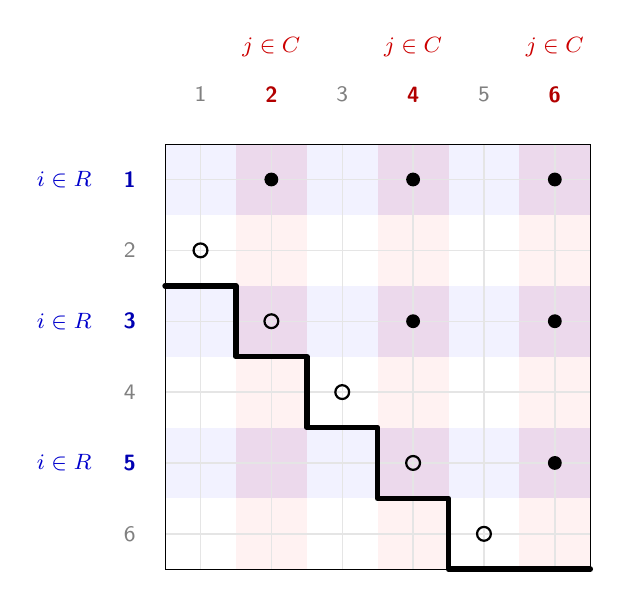
\begin{tikzpicture}[
    scale=0.9,
    grid line/.style={draw=gray!20, line width=0.5pt},
    hessenberg line/.style={draw=black, line width=2pt, line cap=round, line join=round},
    row band/.style={fill=blue!5},
    col band/.style={fill=red!5},
    cross cell/.style={fill=violet!15},
    subdiag node/.style={circle, draw=black, thick, inner sep=0pt, minimum size=5pt},
    entry node/.style={circle, fill=black, inner sep=0pt, minimum size=5pt}
]
\def\n{6}
\def\Rlist{1,3,5}
\def\Clist{2,4,6}

% Background bands
\foreach \r in \Rlist {
    \fill[row band] (0.5, -\r+0.5) rectangle (\n.5, -\r-0.5);
    \node[anchor=east, blue!80!black, font=\footnotesize] at (-0.4, -\r) {$i \in R$};
}
\foreach \c in \Clist {
    \fill[col band] (\c-0.5, -0.5) rectangle (\c+0.5, -\n.5);
    \node[anchor=south, red!80!black, font=\footnotesize] at (\c, 0.6) {$j \in C$};
}

% Intersection cells
\foreach \r in \Rlist {
    \foreach \c in \Clist {
        \fill[cross cell] (\c-0.5, -\r+0.5) rectangle (\c+0.5, -\r-0.5);
    }
}

% Labels
\foreach \k in {1,...,\n} {
    \let\rstyle\relax \def\rcolor{gray}
    \foreach \x in \Rlist { \ifnum\x=\k \global\def\rstyle{\bfseries} \global\def\rcolor{blue!70!black} \fi }
    \node[font=\sffamily\footnotesize\rstyle, color=\rcolor] at (0, -\k) {\k};
    \let\cstyle\relax \def\ccolor{gray}
    \foreach \x in \Clist { \ifnum\x=\k \global\def\cstyle{\bfseries} \global\def\ccolor{red!70!black} \fi }
    \node[font=\sffamily\footnotesize\cstyle, color=\ccolor] at (\k, 0.2) {\k};
}

% Grid
\draw[grid line] (0.5, -0.5) grid (\n.5, -\n.5);
\draw[black, thin] (0.5, -0.5) rectangle (\n.5, -\n.5);

% Hessenberg barrier
\draw[hessenberg line]
    (0.5, -2.5)
    \foreach \k in {1,...,4} {
        -- (\k.5, -\k.5-1)
        -- (\k.5, -\k.5-2)
    }
    -- (6.5, -6.5);

% Nonzeros
\foreach \k in {1,...,5} {
    \node[subdiag node] at (\k, -\k-1) {};
}
\foreach \r in \Rlist {
    \foreach \c in \Clist {
        \pgfmathparse{int(\r<=\c)}
        \ifnum\pgfmathresult=1
            \node[entry node] at (\c, -\r) {};
        \fi
    }
}
\end{tikzpicture}
\caption{Support pattern of $Q_6(\{2, 4\})$, the matrix-side counterpart of
Figure~\ref{fig:digraph-anatomy}. The thick boundary marks the upper
Hessenberg band; open circles ($\circ$) are the mandatory subdiagonal
spine entries; solid dots ($\bullet$) are overlay nonzeros at the
intersections (purple) of active rows (blue) and active columns (red).
The Bridge theorem says these are exactly the nonzero entries of any
unreduced $Q_n(\theta)$ with $S(\theta) = \{2, 4\}$.}
\label{fig:matrix_pattern}
\end{figure}
\FloatBarrier

\begin{example}[$n = 5$, $S = \{2\}$]\label{ex:D5S2}
\leanmargin{example\_D5\_S2}{PaperExamples.lean\#L131}
The angle vector $\theta = (\pi/2, \pi/4, \pi/2, \pi/2)$ gives:
\[
Q = \begin{pmatrix}
0 & \tfrac{1}{\sqrt{2}} & 0 & 0 & \tfrac{1}{\sqrt{2}} \\
-1 & 0 & 0 & 0 & 0 \\
0 & -\tfrac{1}{\sqrt{2}} & 0 & 0 & \tfrac{1}{\sqrt{2}} \\
0 & 0 & -1 & 0 & 0 \\
0 & 0 & 0 & -1 & 0
\end{pmatrix},
\qquad
A = \begin{pmatrix}
0 & 1 & 0 & 0 & 1 \\
1 & 0 & 0 & 0 & 0 \\
0 & 1 & 0 & 0 & 1 \\
0 & 0 & 1 & 0 & 0 \\
0 & 0 & 0 & 1 & 0
\end{pmatrix}.
\]
The Hamilton cycle is $1 \to 5 \to 4 \to 3 \to 2 \to 1$. Since
$R = \{1, 3\}$ and $C = \{2, 5\}$ are disjoint, the digraph is loopless
(Figure~\ref{fig:D5S2}); $A$ is exactly the support pattern predicted by
Theorem~\ref{thm:bridge}.
\end{example}

\begin{figure}[htbp]
\centering
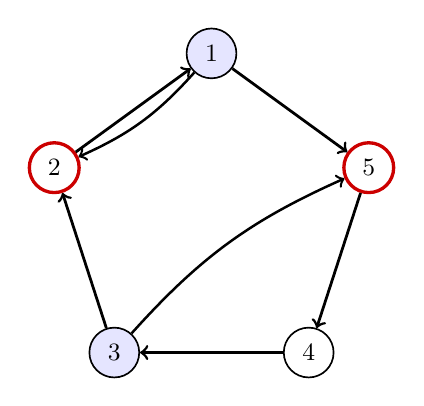
\begin{tikzpicture}[
  v/.style={circle, draw=black, line width=0.6pt, inner sep=1.2pt,
            minimum size=18pt, font=\small},
  cyc/.style={->, line width=1.0pt, draw=black},
  extra/.style={->, line width=0.9pt, draw=black},
  Rnode/.style={fill=blue!10},
  Cnode/.style={draw=red!80!black, line width=1.2pt}
]
\node[v,Rnode] (1) at ( 90:2.1) {1};
\node[v,Cnode] (5) at ( 18:2.1) {5};
\node[v]       (4) at (-54:2.1) {4};
\node[v,Rnode] (3) at (-126:2.1) {3};
\node[v,Cnode] (2) at (162:2.1) {2};

\draw[cyc] (1) -- (5);
\draw[cyc] (5) -- (4);
\draw[cyc] (4) -- (3);
\draw[cyc] (3) -- (2);
\draw[cyc] (2) -- (1);

\draw[extra, bend left=12] (1) to (2);
\draw[extra, bend left=12] (3) to (5);
\end{tikzpicture}
\caption{The loopless support digraph $D_5(\{2\})$. Active rows $R = \{1,3\}$
(blue fill) and active columns $C = \{2,5\}$ (red outline) are disjoint.}
\label{fig:D5S2}
\end{figure}
\FloatBarrier

\begin{theorem}[Rigidity]\label{thm:rigid}
\leanmargin{rigid}{Combinatorial/Rigidity.lean\#L331}
Let $S, S' \subseteq [n-1]$ with $|S|, |S'| \ge 2$. If $D_n(S) \cong D_n(S')$
as digraphs, then $S = S'$.
\end{theorem}

\begin{proof}[Proof sketch]
The key combinatorial fact is the \emph{cut lemma}: in $D_n(S)$, the only
arc from $\{k{+}1, \dots, n\}$ to $\{1, \dots, k\}$ is the spine arc
$k{+}1 \to k$. This forces every isomorphism to fix the unique directed
Hamilton cycle $1 \to n \to n{-}1 \to \cdots \to 2 \to 1$. A pigeonhole
argument on the cut, combined with degree analysis at the
maximum-in-degree vertex (which is $n$ when $|S| \ge 2$), forces the
isomorphism to fix $n$, after which a downward induction along the cycle
forces the identity. The case $|S| = 1$ is the only failure: the cyclic
rotation $\rho^t$ exhibits $D_n(\{t\}) \cong D_n(\{n - t\})$, with no
further coincidences.
\end{proof}

\begin{example}[$n = 5$, $S = \{1, 3\}$]\label{ex:D5S13}
\leanmargin{example\_D5\_S13}{PaperExamples.lean\#L186}
A two-element example illustrating Theorem~\ref{thm:rigid}: any
$D_5(S')$ isomorphic to $D_5(\{1,3\})$ must have $S' = \{1, 3\}$. The
angle vector $\theta = (\pi/4, \pi/2, \pi/4, \pi/2)$ gives:
\[
Q = \begin{pmatrix}
\tfrac{1}{\sqrt{2}} & 0 & \tfrac{1}{2} & 0 & \tfrac{1}{2} \\
-\tfrac{1}{\sqrt{2}} & 0 & \tfrac{1}{2} & 0 & \tfrac{1}{2} \\
0 & -1 & 0 & 0 & 0 \\
0 & 0 & -\tfrac{1}{\sqrt{2}} & 0 & \tfrac{1}{\sqrt{2}} \\
0 & 0 & 0 & -1 & 0
\end{pmatrix},
\qquad
A = \begin{pmatrix}
1 & 0 & 1 & 0 & 1 \\
1 & 0 & 1 & 0 & 1 \\
0 & 1 & 0 & 0 & 0 \\
0 & 0 & 1 & 0 & 1 \\
0 & 0 & 0 & 1 & 0
\end{pmatrix}.
\]
Here $R \cap C = \{1\}$, so there is exactly one self-loop at vertex~$1$
(Figure~\ref{fig:D5S13}).
\end{example}

\begin{figure}[htbp]
\centering
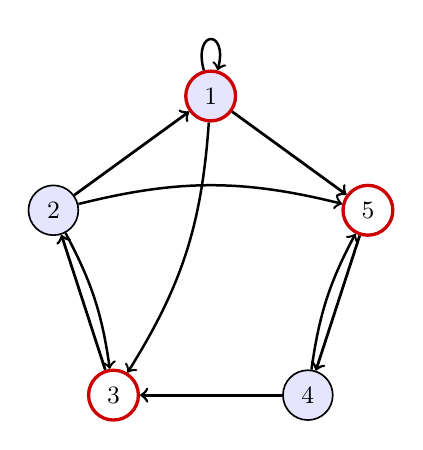
\begin{tikzpicture}[
  v/.style={circle, draw=black, line width=0.6pt, inner sep=1.2pt,
            minimum size=18pt, font=\small},
  cyc/.style={->, line width=1.0pt, draw=black},
  extra/.style={->, line width=0.9pt, draw=black},
  Rnode/.style={fill=blue!10},
  Cnode/.style={draw=red!80!black, line width=1.2pt},
  RCnode/.style={fill=blue!10, draw=red!80!black, line width=1.2pt}
]
\node[v,RCnode] (1) at ( 90:2.1) {1};
\node[v,Cnode]  (5) at ( 18:2.1) {5};
\node[v,Rnode]  (4) at (-54:2.1) {4};
\node[v,Cnode]  (3) at (-126:2.1) {3};
\node[v,Rnode]  (2) at (162:2.1) {2};

\draw[cyc] (1) -- (5);
\draw[cyc] (5) -- (4);
\draw[cyc] (4) -- (3);
\draw[cyc] (3) -- (2);
\draw[cyc] (2) -- (1);

\draw[extra, loop above] (1) to (1);
\draw[extra, bend left=14] (1) to (3);
\draw[extra, bend left=10] (2) to (3);
\draw[extra, bend left=14] (2) to (5);
\draw[extra, bend left=10] (4) to (5);
\end{tikzpicture}
\caption{The support digraph $D_5(\{1,3\})$. Since $R \cap C = \{1\}$, there
is exactly one self-loop at vertex~$1$.}
\label{fig:D5S13}
\end{figure}
\FloatBarrier

\begin{theorem}[Classification]\label{thm:classification}
\leanmargin{classification}{Classification.lean\#L54}
Fix $n \ge 2$. The classification of support digraphs of unreduced
orthogonal upper Hessenberg matrices is the conjunction:
\begin{enumerate}[label=\textup{(\arabic*)}]
\item \textup{(realizability)} every $S \subseteq [n-1]$ is of the form
  $S(\theta)$ for some $\theta \in \Theta_n$;
\item \textup{(bridge)} for every $\theta$, the support of $Q_n(\theta)$
  equals $D_n(S(\theta))$;
\item \textup{(rigidity)} for every $S, S'$ with $|S|, |S'| \ge 2$,
  $D_n(S) \cong D_n(S') \Rightarrow S = S'$.
\end{enumerate}
\end{theorem}

The classification declaration is a one-line term-level packaging of three
independently-proved components; it adds no mathematical content and exists
only so the paper has a single Lean handle to cite. Realizability is
witnessed by the explicit angle choice $\theta_k = \pi/4$ if $k+1 \in S$,
$\theta_k = \pi/2$ otherwise; this gives $\sin \theta_k \ne 0$ always and
$\cos\theta_k \ne 0$ exactly on $S$.


\begin{theorem}[Connected count]\label{thm:count}
\leanmargin{card\_isoClasses\_quot}{Combinatorial/ClassCount.lean\#L268}
For $n \ge 2$, the number of non-isomorphic weakly connected support
digraphs of $n \times n$ unreduced orthogonal upper Hessenberg matrices is
\[
  N_n \;=\; 2^{\,n-1} \;-\; \Big\lfloor \tfrac{n-1}{2} \Big\rfloor.
\]
\end{theorem}

\begin{theorem}[Loopless count]\label{thm:count-loopless}
\leanmargin{card\_looplessClasses\_quot}{Combinatorial/ClassCount.lean\#L526}
For $n \ge 3$, the number of non-isomorphic loopless connected support
digraphs is
\[
  N_n^{\mathrm{loopless}} \;=\; F_{n-1} \;-\; \Big\lfloor \tfrac{n-3}{2} \Big\rfloor,
\]
where $F_k$ is the $k$-th Fibonacci number ($F_0 = 0$, $F_1 = 1$).
\end{theorem}

\begin{proof}[Proof sketch \textup{(both counts)}]
Both counts follow the same template: \emph{labeled} configurations are
subsets $S \subseteq [n-1]$ (resp.\ $S \subseteq \{2, \dots, n-2\}$ with
no consecutive elements, the loopless characterisation). The number of
labeled configurations is $2^{n-1}$ (resp.\ $F_{n-1}$ via the standard
Fibonacci-counts-binary-strings bijection). Subsets with $|S| \ge 2$ are
rigid (Theorem~\ref{thm:rigid}), so each is its own isomorphism class.
The empty subset is rigid alone. The $|S| = 1$ subsets pair up under
$\{t, n-t\}$, contributing $\lceil(n-1)/2\rceil$ (resp.\
$\lceil(n-3)/2\rceil$) classes.
\end{proof}

